\section{Auswertung}
\label{sec:Auswertung}
Alle Berechnungen werden mit dem Programm \glqq Numpy" \cite{numpy}, die Unsicherheiten mit dem Modul \glqq Uncertainties" \cite{uncertainties}, die Ausgleichsrechnungen mit dem Modul \glqq Scipy" \cite{scipy} durchgeführt und die grafischen Darstellungen über das Modul \glqq Matplotlib" \cite{matplotlib} erstellt.


\subsection{Invertierender-Linearverstärker}
\noindent Die Daten werden wie in Abschnitt \ref{sub:Intlin} beschrieben aufgenommen 
und sind in Tabelle \ref{tab:m1}, \ref{tab:m2} und \ref{tab:m3} zu finden.
\newline \newline
\FloatBarrier
\noindent Die Werte werden doppeltlogarithmisch geplottet 
(siehe Abbildung \ref{fig:int100}, \ref{fig:int150} und \ref{fig:int47}).
Die Leerlaufverstärkung $V_0$ wird bestimmt, 
indem durch das Plateau mit einer Konstante gefittet wird 
(siehe Tabelle \ref{tab:Leerlaufverstarkung}):

\begin{table}
    \centering
    \sisetup{table-format = 1.2}
    \begin{tabular}{c c c c}
        \toprule
        $R_2$ in $\qty{}{\kilo\ohm}$ & $V_{0\text{,ideal}} = \frac{R_2}{R_1}$ & $V_0$ \\
        \midrule   
        100 &   100 &   94,244604316546770 \pm 0,000000000000004    \\
        150 &   150 &   140,9 \pm 0,8   \\
        47  &   47  &   45,20 \pm 0,12  \\
        \bottomrule   
    \end{tabular}
    \caption{Die Leerlaufverstärkung des invertierenden Linearverstärkers.}
    \label{tab:Leerlaufverstarkung}
\end{table}
\FloatBarrier
\FloatBarrier
\noindent Die abfallende Kurve wird mit 
\begin{equation*}
    V_0(f) = a f^b
\end{equation*}
\noindent gefittet.
Damit ist die Grentfrequenz 
\begin{equation*}
    f_\text{grenz} = \sqrt[b]{\frac{V_0}{\sqrt{2} a }}.
\end{equation*}
\noindent Das Bandbreitenprodukt wird über 
\begin{equation*}
    GBP= V_0 \cdot f_\text{grenz}
\end{equation*}
\noindent berechnet:

\begin{table}
    \centering
    \sisetup{table-format = 1.2}
    \begin{tabular}{c c c c c}
        \toprule
        $R_2$ in $\qty{}{\kilo\ohm}$ & $a$  & $b$  & $f_\text{grenz}$ in $\qty{}{\kilo \hertz}$ & $GBP$ in $\qty{e5}{\kilo \hertz}$  \\
        \midrule   
        100 &    $(2,9 \pm 1,9)\cdot 10^{6}$ & $-1,17 \pm 0,07$ & $9 \pm 7  $ & $9 \pm 7$ \\
        150 &    $(3,9 \pm 1,4)\cdot 10^{4}$ & $-0,69 \pm 0,04$ & $6 \pm 4  $ & $8 \pm 6$ \\
        47  &    $(6,3 \pm 3,1)\cdot 10^{3}$ & $-0,56 \pm 0,05$ & $13 \pm 16$ & $6 \pm 7$ \\
        \bottomrule   
    \end{tabular}
    \caption{Die Fitparameter, Grentfrequenzen und Bandbreitenprodukte des invertierenden Linearverstärkers.}
    \label{tab:int_fit}
\end{table}

\begin{figure}
    \centering
    \includegraphics[width=\textwidth]{build/int100.pdf}
    \caption{Die Messwerte und Ausgleichsrechnungen 
    des invertierenden Linearverstärkers für $R_2=\qty{100}{\kilo\ohm}$.}
    \label{fig:int100}
\end{figure}
\begin{figure}
    \centering
    \includegraphics[width=\textwidth]{build/int150.pdf}
    \caption{Die Messwerte und Ausgleichsrechnungen 
    des invertierenden Linearverstärkers für $R_2=\qty{150}{\kilo\ohm}$.}
    \label{fig:int150}
\end{figure}
\begin{figure}
    \centering
    \includegraphics[width=\textwidth]{build/int47.pdf}
    \caption{Die Messwerte und Ausgleichsrechnungen 
    des invertierenden Linearverstärkers für $R_2=\qty{47}{\kilo\ohm}$.}
    \label{fig:int47}
\end{figure}
\FloatBarrier
%%%%%%%%%%%%%%%%%%%%%%%%%%%%%%%%%%%%%%%
Als nächtes wird die Phasenverschiebung $\phi$ gegenüber der Frequenz $f$ aufgetragen 
(siehe Abbildung \ref{fig:int100f}, \ref{fig:int150f} und \ref{fig:int47f}). 
Diese ist annähernd bei 180 und bleibt konstant, 
sinkt jedoch ab einer Frequenz mit steigenden Frequenzen ab.

\begin{figure}
    \centering
    \includegraphics[width=\textwidth]{build/int_f100.pdf}
    \caption{Die Phasenverschiebung $\phi$ halblogarithmisch aufgetragen gegen die Frequenz $f$
    des invertierenden Linearverstärkers für $R_2=\qty{100}{\kilo\ohm}$.}
    \label{fig:int100f}
\end{figure}
\begin{figure}
    \centering
    \includegraphics[width=\textwidth]{build/int_f150.pdf}
    \caption{Die Phasenverschiebung $\phi$ halblogarithmisch aufgetragen gegen die Frequenz $f$
    des invertierenden Linearverstärkers für $R_2=\qty{150}{\kilo\ohm}$.}
    \label{fig:int150f}
\end{figure}
\begin{figure}
    \centering
    \includegraphics[width=\textwidth]{build/int_f47.pdf}
    \caption{Die Phasenverschiebung $\phi$ halblogarithmisch aufgetragen gegen die Frequenz $f$
    des invertierenden Linearverstärkers für $R_2=\qty{47}{\kilo\ohm}$.}
    \label{fig:int47f}
\end{figure}
%%%%%%%%%%%%%%%%%%%%%%%%%%%%%%%%%%%%%%%%%%%%%%%%%%%%%%%%%%%%%%%%%%%%%%%%%%%%%%%%%%%%%%%%%%%%%%%%%%%%%%%%%%%%%%%%%%%%%%%%%%%%
%%%%%%%%%%%%%%%%%%%%%%%%%%%%%%%%%%%%%%%%%%%%%%%%%%%%%%%%%%%%%%%%%%%%%%%%%%%%%%%%%%%%%%%%%%%%%%%%%%%%%%%%%%%%%%%%%%%%%%%%%%%%%%%%%%%%%%5
\FloatBarrier
\subsection{Umkehr-Integrator}
\label{sub:aus_int}
Die Werte für den Umkehr-Integrator werden wie in Abschnitt \label{sub:Um_Int} beschrieben aufgenommen
(siehe Tabelle \ref{tab:umint}).
\newline \newline
Die Verstärkung wird gegen die Frequenz doppeltlogarithmisch geplottet (siehe Abbildung \ref{fig:umint})
und mit 
\begin{equation*}
    V(f) = a f^b
\end{equation*}
\noindent gefittet:
\begin{equation}
    a= 78 \pm 5 \quad \text{und} \quad
    b = -0.841\pm 0.019.
\end{equation}

\begin{figure}
    \centering
    \includegraphics[width=\textwidth]{build/umint.pdf}
    \caption{ Die Verstärkung gegen die Frequenz doppeltlogarithmisch geplottet 
    und die dazugehörige Ausgleichsrechnung für den Umkehr-Integrator.}
    \label{fig:umint}
\end{figure}
\FloatBarrier
\noindent Der Umkehr-Integrator wird mit sinusförmige,
dreieckförmige und rechteckförmige Einganssignalen betrieben und die Ausgangssignale auf dem Oszilloskop
angezeigt (siehe Abbildung \ref{fig:int_os}).

\begin{figure}
    \centering
    \begin{subfigure}[b]{0.5\textwidth}
        \centering
        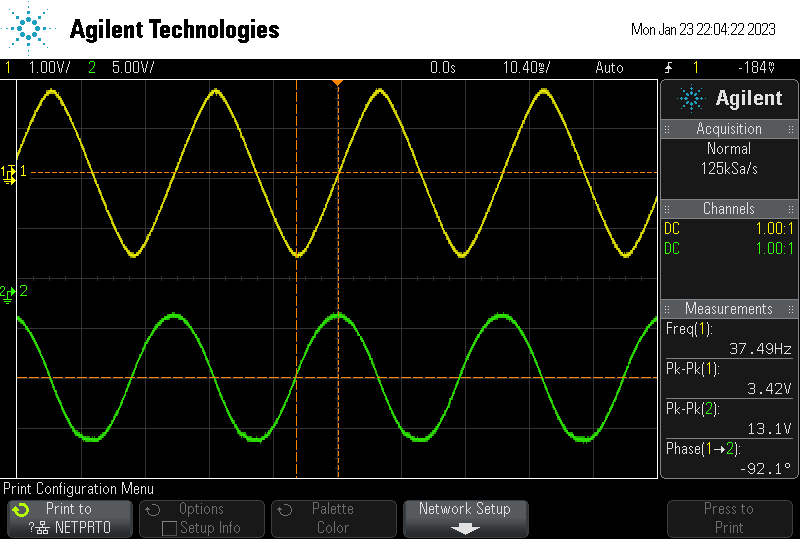
\includegraphics[width=\textwidth]{usb/Int_Sin.png}
        \caption{sinusförmiges Einganssignal}
    \end{subfigure}
    \begin{subfigure}[b]{0.5\textwidth}
        \centering
        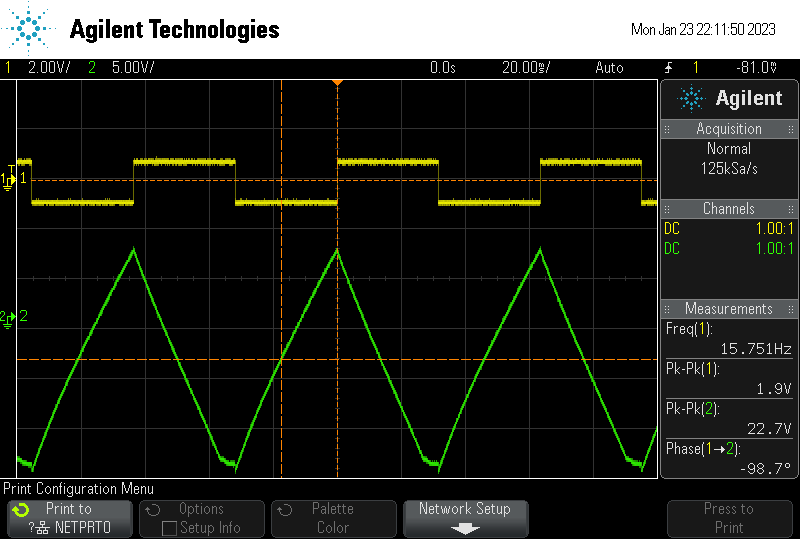
\includegraphics[width=\textwidth]{usb/Int_Recht.png}
        \caption{rechteckförmiges Einganssignal}
    \end{subfigure}

    \begin{subfigure}[b]{0.5\textwidth}
        \centering
        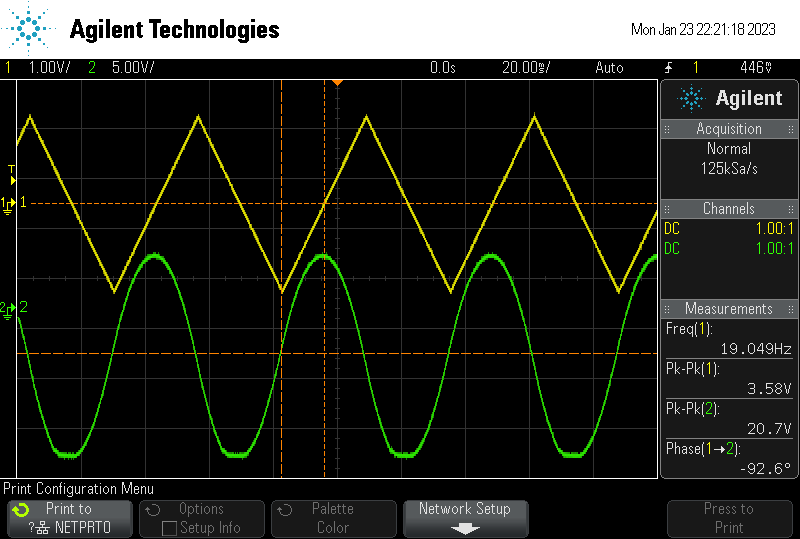
\includegraphics[width=\textwidth]{usb/Int_Drei.png}
        \caption{dreieckförmiges Einganssignal}
    \end{subfigure}
       \caption{Das Einganssignal und Ausgangssignal auf dem Umkehr-Integrator.}
       \label{fig:int_os}
\end{figure}
%%%%%%%%%%%%%%%%%%%%%%%%%%%%%%%%%%%%%%%%%%%%%%%%%%%%%%%%%%%%%%%%%%%%%%%%%%%%%%%%%%%%%%%%%%%%%%%%%%%%%
%%%%%%%%%%%%%%%%%%%%%%%%%%%%%%%%%%%%%%%%%%%%%%%%%%%%%%%%%%%%%%%%%%%%%%%%%%%%%%%%%%%%%%%%%%%%%%%%%%%%%%%
\FloatBarrier
\subsection{Invertierender Differenzierer}
Die Durchführung und Auswertung erfolgt analog zur Abschnitt \ref{sub:aus_int}.
Die Messwerte sind in Tabelle \ref{tab:dif} zu finden und der Fit in Abbildung \ref{fig:dif}:
\begin{equation}
    a =  0.0092 \pm 0.0009 \quad \text{und} \quad
    b =  1.033 \pm 0.016 .
\end{equation}

\begin{figure}
    \centering
    \includegraphics[width=\textwidth]{build/dif.pdf}
    \caption{ Die Verstärkung gegen die Frequenz doppeltlogarithmisch geplottet 
    und die dazugehörige Ausgleichsrechnung für den Invertierenden Differenzierer.}
    \label{fig:dif}
\end{figure}
\FloatBarrier
\noindent Der invertierenden Differenzierer wird ebenfalls mit sinusförmige,
dreieckförmige und rechteckförmige Einganssignalen betrieben und die Ausgangssignale auf dem Oszilloskop
angezeigt (siehe Abbildung \ref{fig:dif_os}).

\begin{figure}
    \centering
    \begin{subfigure}[b]{0.5\textwidth}
        \centering
        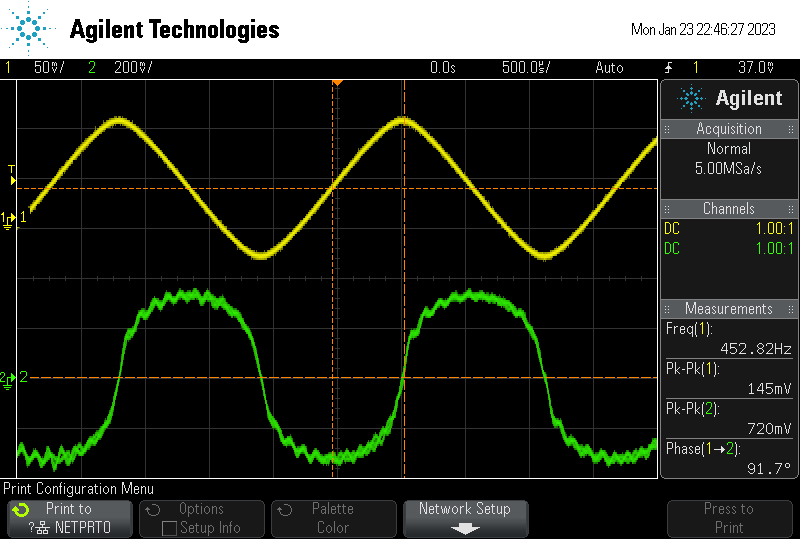
\includegraphics[width=\textwidth]{usb/Dif_Sin.png}
        \caption{sinusförmiges Einganssignal}
    \end{subfigure}
    \begin{subfigure}[b]{0.5\textwidth}
        \centering
        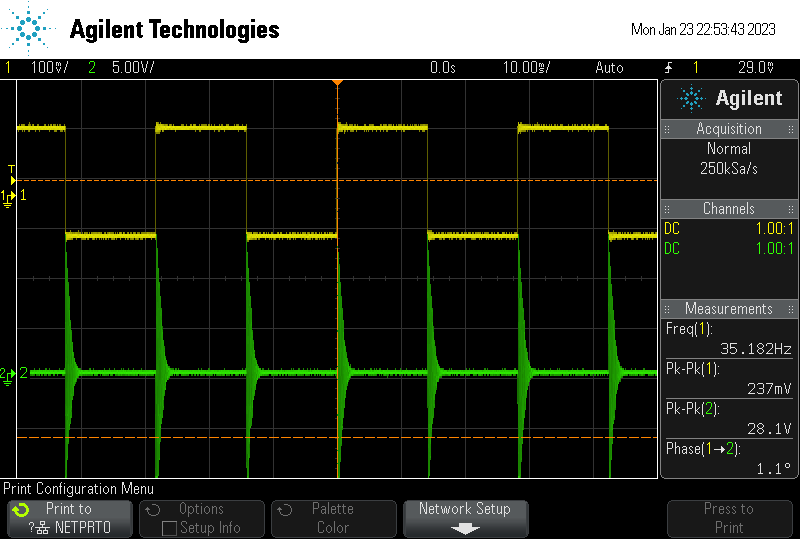
\includegraphics[width=\textwidth]{usb/Dif_Recht.png}
        \caption{rechteckförmiges Einganssignal}
    \end{subfigure}

    \begin{subfigure}[b]{0.5\textwidth}
        \centering
        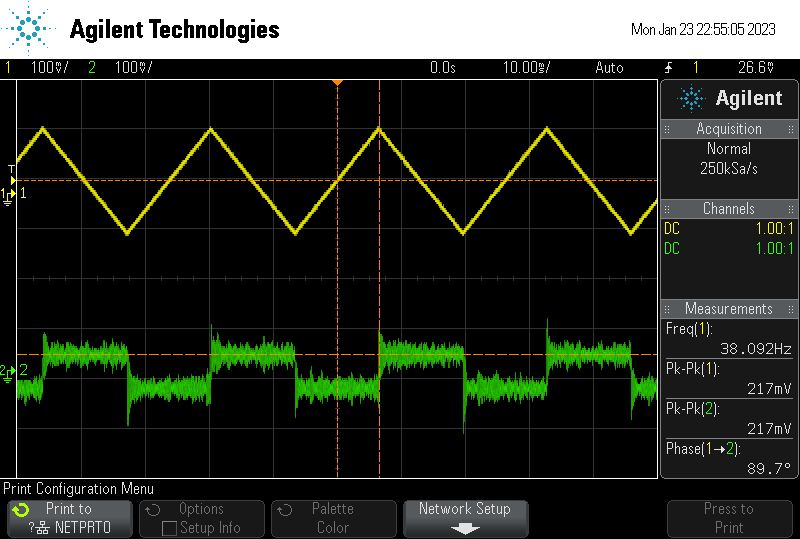
\includegraphics[width=\textwidth]{usb/Dif_Drei.png}
        \caption{dreieckförmiges Einganssignal}
    \end{subfigure}
       \caption{Das Einganssignal und Ausgangssignal auf dem invertierenden Differenzierer.}
       \label{fig:dif_os}
\end{figure}
%%%%%%%%%%%%%%%%%%%%%%%%%%%%%%%%%%%%%%%%%%%%%%%%%%%%%%%%%%%%%%%%%%%%%%%%%%%%%%%%%%%%%%%%%%%%%%%%%%%%%%%%%%%%%%
%%%%%%%%%%%%%%%%%%%%%%%%%%%%%%%%%%%%%%%%%%%%%%%%%%%%%%%%%%%%%%%%%%%%%%%%%%%%%%%%%%%%%%%%%%%%%%%%%%%%%%%%%%%%%%%%%%%%%%%%%
\FloatBarrier
\subsection{Nicht invertierender Schmitt-Trigger}
Wie in Abschnitt \ref{sub:schmitt} geschrieben werden die Einganssignale und Ausgangssignale
auf dem Oszilloskop angezeigt (siehe Abbildung \ref{fig:schmitt}):
Der Abbildung wird die Kippspannung $U_K = \qty{-1.37}{\V}$ 
und die Spannung $U_\text{A, min} = \qty{-14.48}{\V}  $ entnommen.

Der Theorie-Wert wird mit Gl. \ref{eq:schmitt} berechnet $U_\text{K,theo} = \qty{-1.448}{\V}$

\begin{figure}
    \centering
    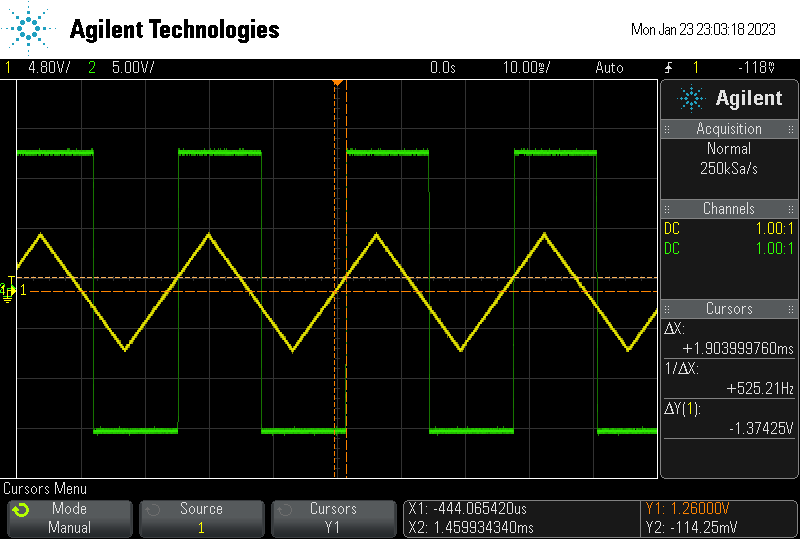
\includegraphics[width=\textwidth]{usb/Trigger.png}
    \caption{ Das dreieckförmige Einganssignal und das entsprechende Ausgangssignal
    des Schmitt-Triggers.}
    \label{fig:schmitt}
\end{figure}
\FloatBarrier
%%%%%%%%%%%%%%%%%%%%%%%%%%%%%%%%%%%%%%%%%%%%%%%%%%%%%%%%%%%%%%%%%%%%%%%%%%%%%%%%%%%%%%%%%%%%%%%%%%%%%%%%%%%%%%%%%%%%%%%%%%%%%
%%%%%%%%%%%%%%%%%%%%%%%%%%%%%%%%%%%%%%%%%%%%%%%%%%%%%%%%%%%%%%%%%%%%%%%%%%%%%%%%%%%%%%%%%%%%%%%%
%%%%%%%%%%%%%%%%%%%%%
\subsection{Signalgenerator}
Die Spannung $U_1$ und $U_A$ werden werden wie in Abschnitt \ref{sub:sig} beschrieben aufgenommen
und der Abbildung \ref{fig:sig} entnommen 
und mit den Gleichungen \ref{eq:sig_f} und \ref{eq:sig_a} berechnet (siehe Tabelle \ref{tab:sig}):

\begin{table}
    \centering
    \sisetup{table-format = 1.2}
    \begin{tabular}{c c c c}
        \toprule
        $f$ in $\qty{}{\kilo\hertz}$ & $f_\text{theo}$in $\qty{}{\kilo\hertz}$ 
        & $\frac{U_\text{A,max}}{U_\text{1,max}}$ & $\frac{U_\text{A,theo}}{U_\text{1,theo}} = \frac{R_1}{R_2}$  \\
        \midrule   
        1,7 & 2,5 & 0,2 & 0,1 \\
        \bottomrule   
    \end{tabular}
    \caption{Die Frequenz $f$ und die Amplitude der Dreieckspannung des Signalgenerators.}
    \label{tab:sig}
\end{table}


\begin{figure}
    \centering
    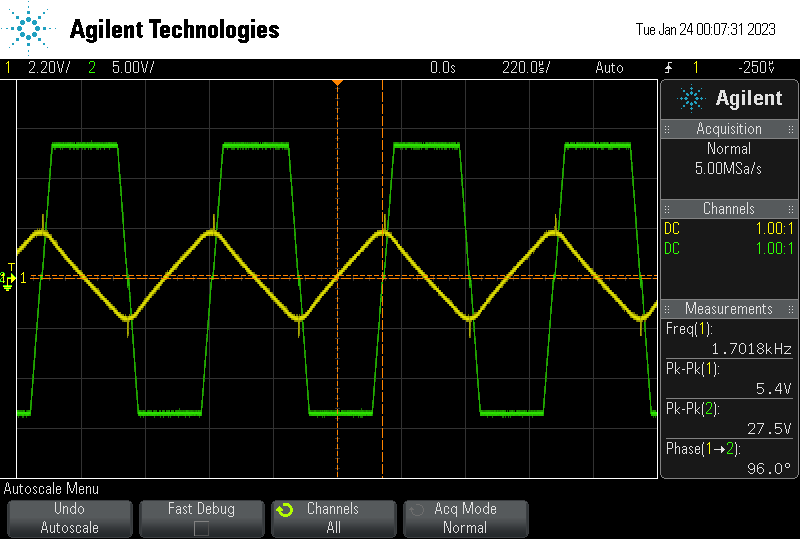
\includegraphics[width=\textwidth]{usb/Signal.png}
    \caption{ Die Spannung $U_1$ und das Ausgangssignal $U_A$ des Signalgenerator.}
    \label{fig:sig}
\end{figure}